\documentclass[conference]{IEEEtran}
\IEEEoverridecommandlockouts

\usepackage{cite}
\usepackage{amsmath,amssymb,amsfonts}
\usepackage{algorithmic}
\usepackage{graphicx}
\usepackage{textcomp}
\usepackage{xcolor}
\usepackage{minted}
\usepackage{array}
\usepackage{float}
\usepackage{multicol}
\usepackage{caption}
\usepackage{ragged2e}
\def\BibTeX{{\rm B\kern-.05em{\sc i\kern-.025em b}\kern-.08em
    T\kern-.1667em\lower.7ex\hbox{E}\kern-.125emX}}
\begin{document}

\title{Image-Based Malware Classification Using Convolutional Neural Networks\\
}

\author{
\IEEEauthorblockN{Raymond Jiang}
\IEEEauthorblockA{\textit{Glen A. Wilson High School} \\
Hacienda Heights, USA \\
raymondjiang0917@gmail.com}
\and
\IEEEauthorblockN{Abdullah Irfan Siddiqui}
\IEEEauthorblockA{\textit{College of Science} \\
California State Polytechnic\\
University at Pomona\\
Pomona, USA\\
abdullahi@cpp.edu}
\and
\IEEEauthorblockN{Srijit Bhattacharya}
\IEEEauthorblockA{\textit{College of Science} \\
California State Polytechnic\\
University at Pomona\\
Pomona, USA\\
srijitb@cpp.edu}
\and
\IEEEauthorblockN{Mohammad Husain}
\IEEEauthorblockA{\textit{College of Science} \\
California State Polytechnic\\
University at Pomona\\
Pomona, USA\\
mihusain@cpp.edu}
}

\maketitle

%---------------------------------------------------------------------------------------------------------------------------------

\begin{abstract}
As the tech world increasingly integrates into our lives, so does the sophistication of malware. Effective malware classification is an important step for the prevention and mitigation of malware as it allows the identification of new threats without reliance on existing malware databases. Traditional techniques, such as manual code analysis, often have significant limitations and can be easily prevented by attackers. This paper proposes a novel approach to malware classification by directly analyzing the malware file itself, bypassing the need for code disassembly. In this approach, malware bytes files are converted to an image which are fed into a Convolutional Neural Network for pattern feature extraction to classify each image in their respective malware classes, completely skipping the need to scan the actual code, rendering code obfuscation ineffective. Our approach demonstrates significant improvements in accurately detecting and classifying new malware threats, with consistent accuracies of 96\%+. Our findings indicated that the use of an CNN model to classify malware types are accurate and are a more dependable way for classification, creating a future possibility to detect newly created malware and take prevention measures early on.
\end{abstract}

\begin{IEEEkeywords}
malware classification, code analysis, malware, Convolution Neural Network (CNN), code obfuscation
\end{IEEEkeywords}

%---------------------------------------------------------------------------------------------------------------------------------

\section{Introduction}
Since the creation of the internet, malicious code has been written to exploit software bugs and perform malicious tasks. The first ever malware written exploited the lack of security in a system called ARPANET\cite{johanna-2024}. However, in its most basic form, malware is just code written that, when executed, performs a specific task, which in most cases is meant for harm\cite{i2}. While software developers are patching these exploits, it becomes a problem when these exploits are found before such developers. This presents the issue of Zero-Day exploits\cite{i3}, allowing attackers to use custom and never-before-seen malware. There are several ways to classify malware; however, each has flaws.

The most common way is code analysis, which involves manually reviewing each malware's code. To start this process, the malware file would often need to decompile the malware file using various applications to access its original code. Similarly, there is static code analysis, in which instead of a human going through code line by line, a program goes through it and identifies possible vulnerabilities in it\cite{i4}. However, this type of analysis can be prevented by code obfuscation, which can prevent disassembles or humans from reading clear code.

Current antivirus programs also use signature-based detection as one of their main lines of defense against malware. Signature-based detection scans through every file signature or a file's information\cite{i5}. It will then match it to a vast database of known malware signatures and determine if it should be blocked from the system. This approach is most commonly used and very effective for various reasons. Its efficiency is unrivaled by other techniques due to its simplicity; it is only a matching system that checks if a particular file is in its malware database. Since it only matches and does not make predictions, this system is highly accurate, making it a trustworthy technique. However, due to its structure, it has a few limitations. Since it only matches malware to a database, the new malware created will only be detected once registered. On top of that, constant updates are required to keep up with the new malware types. 

The technique we will attempt to employ is similar to signature-based detection but without its limitations. We will be training an AI Convolutional Neural Network\cite{i6} to identify malware files. By doing this, our goal is to be able to classify malware whose code is not obfuscated, eliminating the limitation presented by static code analysis. On top of this, by using the CNN model to classify malware, we plan to train on previous databases of malware similar to one of signature-based detection.

%---------------------------------------------------------------------------------------------------------------------------------

\section{Related Works}
This section provides a comprehensive overview of previous research, encompassing different classification techniques mainly regarding using machine learning models as the basis for classification. These studies have contributed heavily into various domains of experimentation including but not limited by: Android, Windows, etc.

    H. AlOmari \textit{et al}  \cite{ALOMARI2023763}  investigates the performance of different machine learning algorithms in detecting various Android-based malware using the CICMalDroid2020 dataset comprised of 11,598 APKs. They used CopperDroid to use dynamic feature extraction on each APK. They preprocessed the data using Synthetic Minority Oversampling Technique (SMOTE) and normalized values via Z-score normalization in preparation for the model. They used various machine learning classifiers such as LightGBM, Random Forest, Extra Trees, Gradient Boosting, Decision Trees, K Neighbors, and Ada Boost in their evaluation. Their results found that the Light Gradient Boosting Machine (LightGBM) algorithm was the most effective, having an F1-score of 94.77\%. The authors have also found that data preprocessing steps, such as data normalization, significantly improved the performance of Logistic Regression. Similarly, SMOTE dealt with class imbalance, which improved the performance of many classifiers.

    A. Wajid \textit{et al} \cite{Wajid_Ahmed_Chaudhry_2024}  explores the different techniques used for code analysis: static, dynamic, and hybrid, using data from previous research papers. The authors compare signature-based analysis (static) and behavior-based analysis (dynamic). Their data comes from papers within the following criteria: relevance, publication year, data validity, methodology, and evaluation. They want their selected papers to (I) be relevant to malware detection using machine learning models in Windows; (II) be published between 2019 - 2023 to be updated enough; (III) have the data used in the experiment must be publically available; (IV)  experiments in each paper must use machine learning algorithms; and lastly (V) have the results of the study must be quantifiable using standard metrics like accuracy. From their observations of the collected articles, the RF algorithm was the most consistent, with accuracy rates varying from 98.63\% to 99.8\%. They also separated these articles into either feature-based or image-based approaches. Feature-based methods extract data from malware binaries, such as PE headers, API calls, opcode sequences, etc., for classification. In contrast, image-based methods convert the malware binary files into images (greyscale or RGB) and use image classification machine learning models. They found that static analysis was often much faster and safer, as it required no actual execution of the file, only looking at the code. However, it had limitations that dynamic analysis picked up on: (I) it could often be prevented via code encryption or other forms of obfuscation; and (II) it could also not observe runtime interactions of the malware. On the other hand, dynamic analysis filled up the flaws left by static analysis, as it required the actual execution of the code in a controlled environment. This allowed models to pick up on its actions and also allowed it to predict and identify new malware types. However, its limitations would be that it was very computationally heavy, as it required running each malware file in a sandbox, which can be time-consuming. They proposed using a hybrid analysis technique, incorporating the pros from each type of analysis and combining them. 

    H. S. Anderson \textit{et al} \cite{Anderson2018EMBERAO}  introduced their dataset called EMBER, an open dataset for machine learning models used regarding Windows malware, specifically, portable executable files. This dataset contains approximately 1.1 million data lines split with an 82:18 training-to-testing data ratio. The 900,000 training samples are split between 300,000 malicious, 300,000 benign or harmless, and 300,000 unlabeled data. The 200,000 testing samples were split into a 50:50 ratio of 100,000 malicious and 100,000 harmless. The data is a collection of JSON lines, in which each line or object contains data about each malware. The format includes sha256, date, label, and raw features. The sha256 contains the sha256 hash of the specific malware file; the date is the estimated date that the malware was first seen, and the label is used to define if the file is malicious, benign, or unlabeled. Their goal for this paper was to contribute to the cyber security industry by providing a massive and open dataset to increase more data within the domain. They built a decision tree baseline model based on LightGBM fed with the EMBER dataset to test the dataset. The model was a gradient-boosted decision tree (GBDT) trained using LightGBM with only default parameters. The results of this model were very promising; it received a high ROC AUC score (0.99821), indicating that it could classify the testing data well. This was compared with MalConv, a deep learning machine learning model with hyper-parameter optimization. This comparison noted that the baseline model trained solely using the EMBER dataset outperformed MalConv. 

    P. Maniriho\textit{ et al} \cite{MANIRIHO2024111921}  conducted a systematic literature review on Windows malware detection techniques. They focused on static, dynamic, and hybrid analysis methods that these articles used as their results. They identified two methods of static analysis: signature-based detection and heuristic-based detection. Signature-based detection relies on an extensive database of malware signatures and uses it to identify existing malware. On the other hand, heuristic-based detection looks at code patterns to check for potential malicious behavior. In the case of dynamic analysis, they have defined it in two categories: behavior-based detection and memory analysis. Behavior-based detection runs the malware program in a controlled system and analyzes its behavior to detect zero-day vulnerabilities. Memory analysis uses dumps to find the program's activities and detect if they are malicious. The third and last technique they reviewed would combine the previous two, called hybrid analysis. Both are combined to improve accuracy through each technique's strengths. The paper mentions primary datasets such as CSDMC2010, MalImg, Microsoft BIG2015, and EMBER, which were all essential in evaluating malware detection techniques in their reviewed papers. These public datasets allow others to reproduce and scale their programs. They also looked at biases that could have affected performance, such as temporal, spatial, and sample size. These biases are essential to consider since they can vastly change an experiment's results and make them less reliable if too large. When measuring the performance of each study's results, they often used standard performance metrics such as accuracy, precision, recall, F1 scores, and AUCROC scores. These scores can show each model's faults and be used to detect them. False negatives and false positives can be harmful in practice, producing skewed or incorrect results. This review provides information on the current and future states of malware detection in Windows, as presented in various studies.

%---------------------------------------------------------------------------------------------------------------------------------

\section{Methodology}

\subsection{The Dataset}
The data used to train and test the convolutional neural network (CNN) were from the malimg dataset\cite{m1}  which consists of 9,339 malware images from 25 different classes.
    
\begin{figure}[htbp]
\centerline{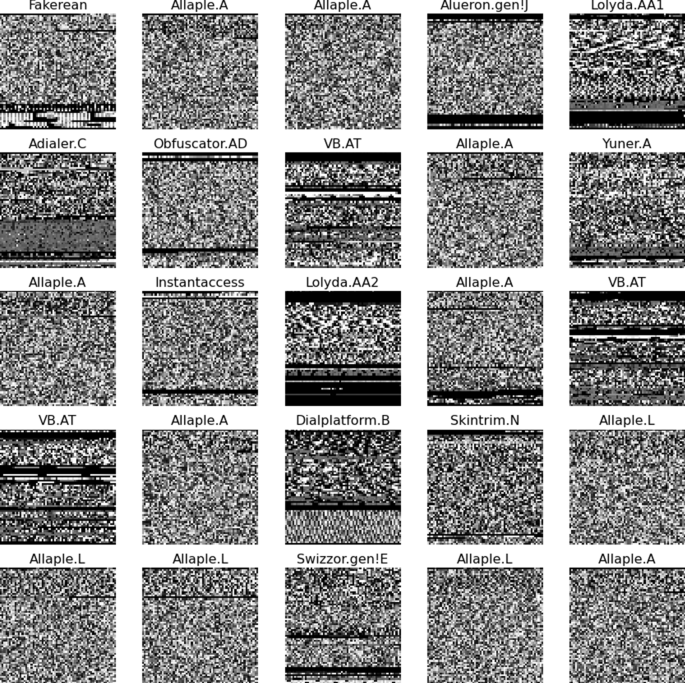
\includegraphics[width=1\linewidth]{images/malImg dataset picture.png}}
\caption{Sample pictures of the malImg dataset from each of the 25 different malware families.}
\label{mf1}
\end{figure}
The classes included:
\begin{table}[htbp]
\caption{List of Malware Families used}
\begin{center}
\begin{tabular}{|c|c|c|}
\hline
VB.AT&Rbot!gen& Skintrim.N\\ \hline 
Yuner.A& Lolyda.AA1& Obfuscator.AD\\ \hline
Swizzor.gen!E& Lolda.AA2& Agent.FYI\\ \hline 
 Swizzor.gen!I&Lolyda.AT& Lolyda.AA3\\ \hline
 Wintrim.BX& Instantaccess& Fakerean\\ \hline
 Malex.gen!J& C2LOP.gen!g& C2LOP.P\\ \hline
 Alueron.gen!J& Allaple.A& Dontovo.A\\ \hline
 Allaple.L& Adialer.C& Dialplatform.B\\ \hline
 Autorun.K& & \\\hline\end{tabular}
\label{mt1}
\end{center}
\end{table}
\subsection{Data Preprocessing}
When presented with such a large dataset, filtering out data and processing it is essential to ensure a model is trained correctly. While not required for the malimg dataset we used in this experiment, a conversion will first need to be done to get the raw file into an image. For example, we would use BYTES files, converting it PNG files used later for model data.

After the conversion process from BYTES to PNG, we used Keras's built-in preprocessing class called ImageDataGenerator(). Since we were importing from a folder,  we would use the method flow\_from\_directory, which ended up looking like this: 

\centering
ImageDataGenerator().flow\_from\_directory(root, target\_size=(64,64), batch\_size=10000)

\begin{table}[htbp]
\caption{Parameters for Preprocessing}
\begin{center}
\begin{tabular}{|c|>{\centering\arraybackslash}p{0.75\linewidth}|}
\hline
\textbf{Parameter}&\textbf{Details}\\ \hline 
root& Specifies the directory of the folder containing classes\\
\hline
target\_size& The size of each image in pixels; in our case, each image was 64 x 64 \\\hline
 batch\_size& The amount of images to be processed; in our case there were 9339 images, so a batch size of 10,000 would be able to load all images\\\hline\end{tabular}
\label{mt2}
\end{center}
\end{table}

We would then use the next() function to iterate through the array of images, separating data into two NumPy arrays, one for the image itself and the other for its class/label name. This is done so that each element in the image corresponds to the same element in the same index of the label array.
\medskip

The result would be two arrays with a total of 9339 data indexes in each:\\
images.shape = (9339, 64, 64, 3)
    \begin{itemize}
  \item 9339 total images
  \item 64 by 64 is the size of each image
  \item  3 colors are used (Red, Green Blue)
\end{itemize}
labels.shape = (9339, 25)
\begin{itemize}
  \item 9339 total images with labels
  \item 25 different labels in total
\end{itemize}
\medskip
Our final step in processing data would be to split data up into proper proportions for model training. We used a 70:30 training-to-testing ratio in this step, using Keras's train\_test\_split() method. This creates four different arrays, similar to the images and labels from above, but split into training and testing.

\begin{table}[htbp]
\caption{Preprocessing Results}
\begin{center}
\begin{tabular}{|c|c|}
\hline
\textbf{Array}&\textbf{Details}\\ \hline 
X\_train& Array of images for training\\
\hline
X\_test& Array of images for testing\\\hline
 Y\_train& Array of labels for training\\\hline
 Y\_test&Array of labels for training\\\hline\end{tabular}
\label{mt3}
\end{center}
\end{table}

This ended with 6537 data values for training and 2802 for testing.

\subsection{Model Structures}
This section examines the various structures/layers of the convolutional neural network model used for testing and provides an overall overview of each structure's purpose.

\begin{table}[H]
\caption{CNN Layers}
\begin{center}
\begin{tabular}{|c|>{\centering\arraybackslash}p{0.6\linewidth}|}
\hline
\textbf{Layer Name}  &\textbf{Layer Details}\\ \hline 
Input & Instantiates a Keras tensor from input\\
\hline
Conv2D & Applies convolutional filters to extract features from input. They are able to extract spatial characteristics from an image.\\\hline
 MaxPooling2D& Reduces dimensions by taking the maximum value over a grid of values\\\hline
 BatchNormalization& Normalizes inputs\\\hline
 Flatten& Converts multidimensional tensor into a single vector\\\hline
 Dense& Used for training and making predictions through interconnnected nodes\\\hline
 Dropout& Randomly drops nodes during training to prevent overfitting\\\hline\end{tabular}
\label{mt4}
\end{center}
\end{table}
\justifying
Using these layers, there were three iterations of structures before we found the most optimal version, a model that did not overfit nor underfit. Underfitting would mean the model could not properly train, with a low accuracy rate during training and testing\cite{m5}. On the other hand, overfitting is the opposite; the model is so close to the training data that the new testing data results in large drops in prediction accuracy\cite{m4}.

\subsubsection{Starter Model}
For this model, we used the following structure:
\begin{table}[H]
\caption{Starter Model Layers/Settings}
\begin{center}
\begin{tabular}{|c|>{\centering\arraybackslash}p{0.6\linewidth}|}
\hline
\textbf{Layer Name}  &\textbf{Layer Parameters}\\ \hline 
Input & (shape=(64, 64, 3))\\
\hline
Conv2D & (32, (3, 3), activation='relu', padding='same')\\\hline
 MaxPooling2D& ((2, 2))\\\hline
 BatchNormalization& NA\\\hline
 Flatten& NA\\\hline
 Dense& (128, activation='relu')\\\hline
 Dropout& (0.5)\\\hline
 Dense&(25, activation='softmax')\\\hline
 model.compile&(optimizer='adam', loss='categorical\_crossentropy', metrics=['accuracy'])\\\hline
 model.fit&(X\_train, Y\_train, epochs=20, batch\_size=64, validation\_data=(X\_test, Y\_test))\\\hline\end{tabular}
\label{mt5}
\end{center}
\end{table}

This model was the starting point for us to find the most optimal parameters for each layer. We would start with the standard values for layers, such as 32 nodes for convolution2d, 128 node dense layer, and a 50\% dropout percentage. The activation functions used were also very standard, with RELU\cite{krishnamurthy-2024} used most of the time and SOFTMAX\cite{wood-2020} used for the ending result layer. We trained this model and found that 20 epochs are enough for the model to develop and prevent overfitting but also long enough to produce results accurately.

\subsubsection{Revised Model}

After solidifying the working features of the starting model, we started to increase and change around values in the layers. We used the following structure for this model:
\begin{table}[H]
\caption{Revised Model Layers/Settings}
\begin{center}
\begin{tabular}{|c|>{\centering\arraybackslash}p{0.6\linewidth}|}
\hline
\textbf{Layer Name}  &\textbf{Layer Parameters}\\ \hline 
Input & (shape=(64, 64, 3))\\
\hline
Conv2D & (32, (3, 3), activation='relu', padding='same')\\ \hline 
 MaxPooling2D&((2, 2))\\ \hline 
 BatchNormalization&NA\\\hline
 Conv2D &(64, (3, 3), activation='relu', padding='same')\\ \hline 
 MaxPooling2D&((2, 2))\\ \hline 
 BatchNormalization&NA\\ \hline 
 Conv2D &(128, (3, 3), activation='relu', padding='same')\\\hline
 MaxPooling2D& ((2, 2))\\\hline
 BatchNormalization& NA\\\hline
 Flatten& NA\\\hline
 Dense& (128, activation='relu')\\\hline
 Dropout& (0.5)\\ \hline 
 Dense&(128, activation='relu')
\\\hline
 Dropout&(0.5)\\\hline
 Dense&(25, activation='softmax')\\\hline
 model.compile&(optimizer='adam', loss='categorical\_crossentropy', metrics=['accuracy'])\\\hline
 model.fit&(X\_train, Y\_train, epochs=20, batch\_size=64, validation\_data=(X\_test, Y\_test))\\\hline\end{tabular}
\label{mt6}
\end{center}
\end{table}

With this model, we aimed to exaggerate as much as we could for the parameters and layers. We added two more convolutional layers, each with twice more than the previous number of nodes (32, 64, 128). In addition, we also added another dense layer with the same number of nodes (128) along with its same dropout percentage (50\%). We kept the same parameters for model compilation and fitting, with adam optimizer and 20 epochs.

\subsubsection{Final Model}

With the revised model telling us the results of an extreme structure, we opted to find the middle ground between the starter and the revised model, ending up with the following structure:
\begin{table}[H]
\caption{Final Model Layers/Settings}
\begin{center}
\begin{tabular}{|c|>{\centering\arraybackslash}p{0.6\linewidth}|}
\hline
\textbf{Layer Name}  &\textbf{Layer Parameters}\\ \hline 
Input & (shape=(64, 64, 3))\\
\hline
Conv2D & (32, (3, 3), activation='relu', padding='same')\\ \hline 
 MaxPooling2D&((2, 2))\\ \hline 
 BatchNormalization&NA\\\hline
 Conv2D &(32, (3, 3), activation='relu', padding='same')\\ \hline 
 MaxPooling2D&((2, 2))\\ \hline 
 BatchNormalization&NA\\\hline
 Flatten& NA\\\hline
 Dense& (128, activation='relu')\\\hline
 Dropout& (0.5)\\ \hline 
 Dense&(128, activation='relu')
\\\hline
 Dropout&(0.5)\\\hline
 Dense&(25, activation='softmax')\\\hline
 model.compile&(optimizer='adam', loss='categorical\_crossentropy', metrics=['accuracy'])\\\hline
 model.fit&(X\_train, Y\_train, epochs=20, batch\_size=64, validation\_data=(X\_test, Y\_test))\\\hline\end{tabular}
\label{mt7}
\end{center}
\end{table}
We opted to use two convolution layers, each remaining with 32 nodes. Two dense layers were kept, each with 128 nodes and a RELU\cite{krishnamurthy-2024} activation, paired with dropout layers of 50\%. We kept the same parameters for model compilation and fitting, with adam optimizer and 20 epochs.

\section{Evaluation}
We will now start to run these models on the dataset specified earlier. As stated previously, these models be of a convolutional neural network style, with its primary purpose to classify malware, which have been converted into images. To evaluate our models, we will be using classification performance metrics such as accuracy, F1-score, recall, and precision.

\subsection{Classification Evaluation Metrics}
To evaluate our models, we will use accuracy, F1-score, recall, precision, and ROC AUC scores. We will also use loss graphs and confusion matrices to view each model's predictions completely. We start by separating each of our predictions into four categories.
\begin{itemize}
\item True Positive (TP): Data labeled to family X are correctly classified as family X.
\item True Negative (TN): Data labeled not family Y are correctly classified as not family Y
\item False Positive (FP): Data labeled to family X are incorrectly classified as family Y
\item False Negative (FN) Data labeled not family Y are incorrectly classified as family Y
\end{itemize}

These categories are the basis of our various evaluation metrics and can be used to determine the performance of each model.

We start by using accuracy as our first metric for each model. This allows us to check each model's ratio of correct predictions to total predictions.
\[ Accuracy = \frac{TP + TN }{TP + TN + FP + FN}\]
Recall will also be used to evaluate each model's ability to predict positive instances. It is the ratio of correct positive predictions to total positives.
\[Recall = \frac{TP}{TP + FN}\]
Precision will also be used, allowing us to evaluate each model's accuracy of positive predictions. It is the ratio of correct positive predictions to total positive predictions.
\[Precision = \frac{TP}{TP + FP}\]
F1-Score will also be used, allowing us to evaluate both precision and recall on the model. This allows us to balance both metrics and not sacrifice one for the other. The formula for F1-score is:
\[F1\mbox{-}Score = 2 \times \frac{Precision \times Recall}{Precision + Recall}\]
Our final evaluation metric will be the ROC-AUC score, which measures each model's ability to distinguish between positive and negative cases. It is the area under the curve (AUC) of a True Positive Rate v False Positive Rate graph, where the best outcome is when the false positive rate (FPR) is at 0 and the true positive rate (TPR) is at 1. The mathematical representation of this score is as following:\cite{aim-2021}
\[
\text{AUC} = \int_{0}^{1} \text{TPR}(\text{FPR}^{-1}(x)) \, dx
\]

We will also use confusion matrices and loss graphs to visualize the model's predicted results and how they correctly evaluate each picture.

%---------------------------------------------------------------------------------------------------------------------------------

\subsection{Accuracy}
\begin{figure}[h]
\begin{minipage}[b]{0.49\linewidth}
  \centering
  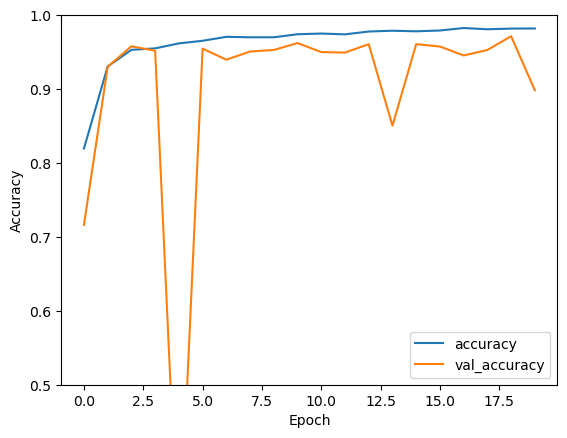
\includegraphics[width=1\linewidth]{images/starter/acc.png}
  \caption{Accuracy Graph of Starter Model}
  \label{afs}
\end{minipage}
\hfill
\begin{minipage}[b]{0.49\linewidth}
  \centering
  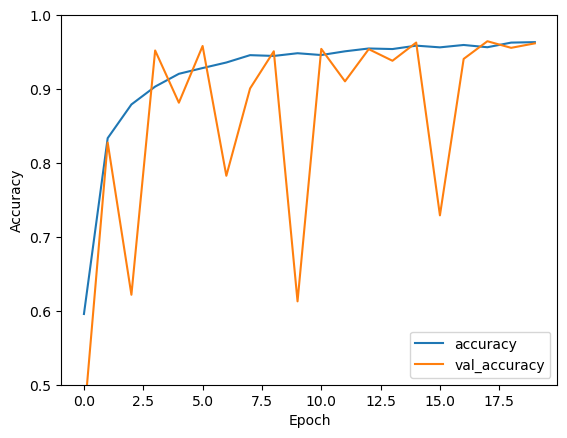
\includegraphics[width=1\linewidth]{images/revise/acc.png}
  \caption{Accuracy Graph of Revised Model}
  \label{afr}
\end{minipage}
\vspace{1em}
\begin{minipage}{\linewidth}
  \centering
  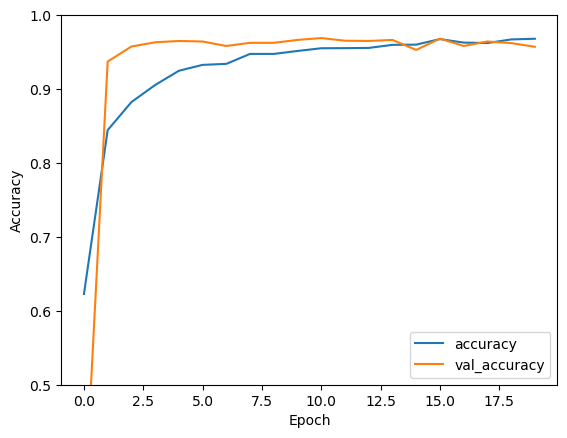
\includegraphics[width=0.5\linewidth]{images/final/acc.png}
  \caption{Accuracy Graph of Final Model}
  \label{aff}
\end{minipage}
\end{figure}
Above are the accuracy vs epoch graphs for the starter (Fig. \ref{afs}), revised (Fig. \ref{afr}), and final (Fig. \ref{aff}) models. Starting, we recognize that the final graph has a near-perfect line for training and validation accuracy without any large fluctuations across epochs. This can show us that this is a near-perfect model for testing, as it will be consistently accurate even with different data. However, in the other two graphs (Fig. \ref{afs} \& \ref{afr}), we can see that the accuracy fluctuates violently, such as in epoch 4 for Fig. \ref{afs}. By these large fluctuations, we can conclude that the starter and revised models must have been over-fitted, which means that the models were too used to the training data, so when introducing the validation set, it could not fully detect them correctly. However, the difference between the two models is the frequency of drops. The revised model's validation accuracy fluctuated much more than the starter model, indicating a stronger sense of overfit. When comparing the code between each model, we can see that with the starter model, it is possible that since there were insufficient training processes, the model could not fully develop and dropped in accuracy in the few times it met new data. However, with the revised model, there were too many additional layers, which proved unnecessary and only led to the model being too close to the training data, aka overfitting.


\subsection{F1-Score, Recall, and Precision}

\begin{table}[H]
    \centering
    \caption{Weighted Averages of F1-Score, Recall, and Precision metrics for each type of model}
    \label{mt}
    \begin{tabular}{|c|c|c|c|} \hline 
         \textbf{Models}&  \textbf{F1-Score}&  \textbf{Recall}& \textbf{Precision}\\ \hline 
         Starter&  0.90&  0.90& 0.93\\ \hline 
         Revised&  0.95&  0.96& 0.95\\ \hline 
         Final&  0.97&  0.97& 0.97\\ \hline
    \end{tabular}
\end{table}

The above table represents all the numerical metrics obtained during the evaluation process: F1-Score, Recall, and Precision. We can see the improvement in each category as the models progress throughout from starter, revised, and final. However, we can see a massive jump in performance between the starter and revised models, an approx 0.05-0.06 increase. This boost can be explained when comparing the differences, in the starter model, there wasn't enough layers (convolutional, dense, batch normalization, etc) while compared to the revised model, there were too many layers. This can also show that it is more preferred to have more layers than not, as you can lose a lot of possible training. The difference between the final and revised models is not a lot, by 0.01-0.02 but it can still show how adding more layers isnt always helpful, in most cases, it can degrade performance.

\subsection{ROC-AUC}
\begin{figure}[H]
  \centering
  \captionsetup{justification=centering}
  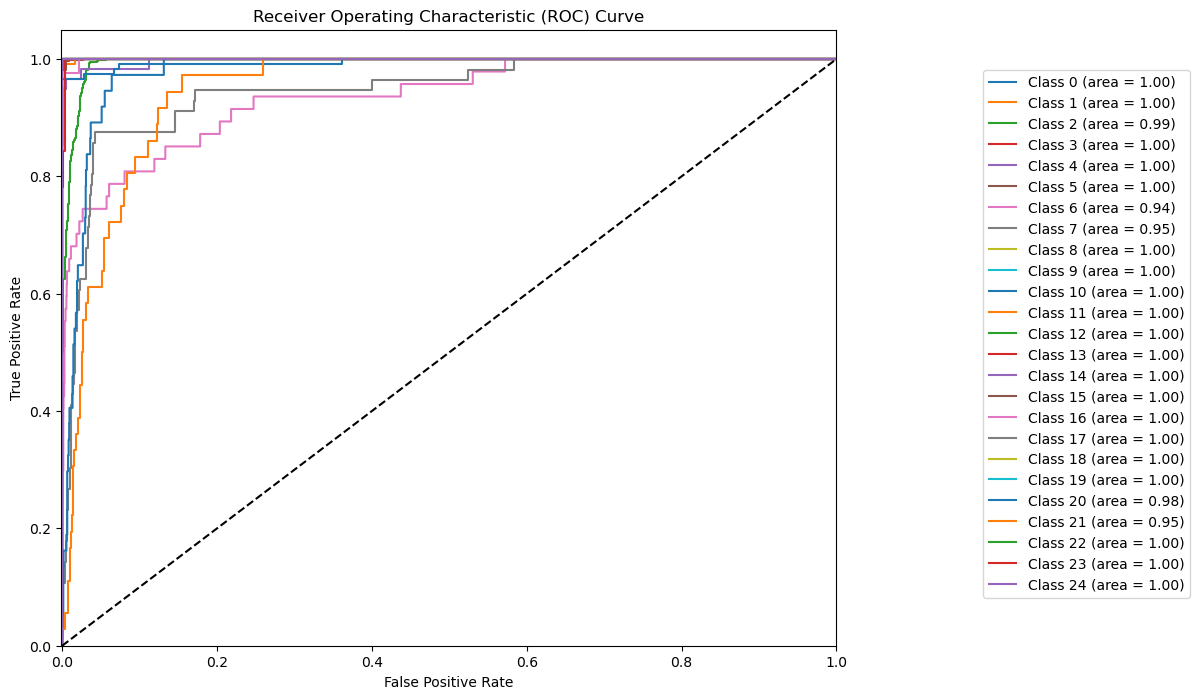
\includegraphics[width=0.8\linewidth]{images/starter/roc.png}
  \caption{AUC-ROC Curve of Starter Model\\AVG ROC AUC: 0.99184}
  \label{afs}
\end{figure}

\begin{figure}[H]
  \centering
  \captionsetup{justification=centering}
  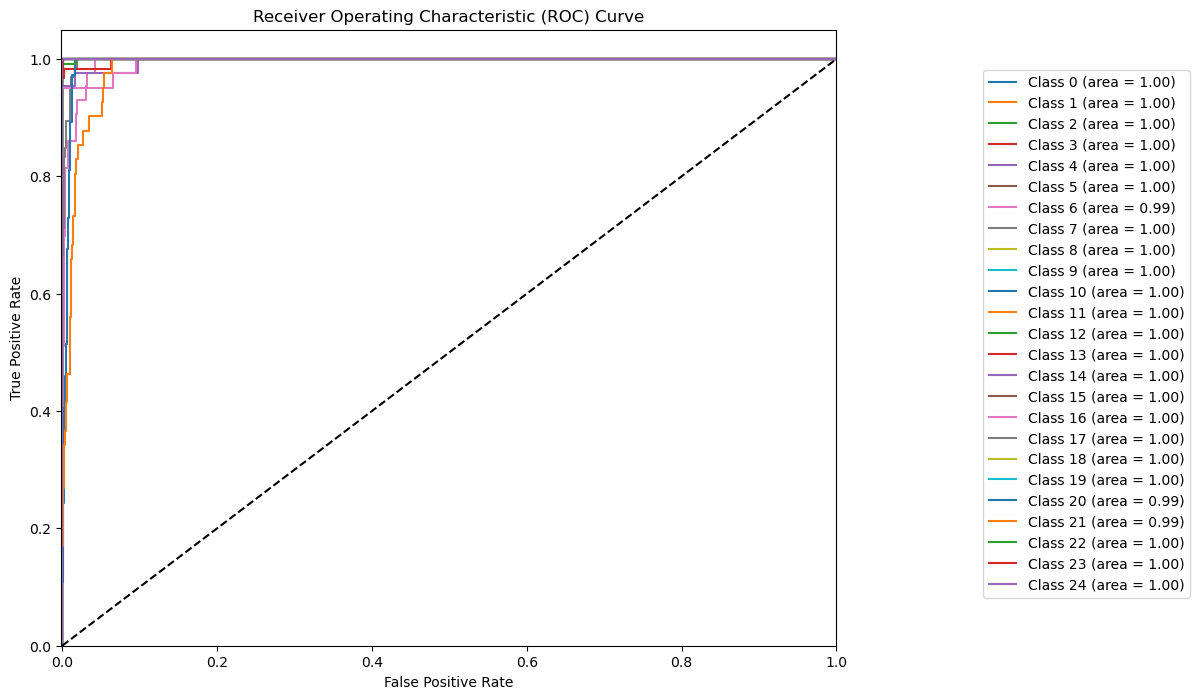
\includegraphics[width=0.8\linewidth]{images/revise/roc.png}
  \caption{AUC-ROC Curve of Revised Model\\AVG ROC AUC: 0.99862}
  
  \label{afr}
\end{figure}

\begin{figure}[H]
  \centering
  \captionsetup{justification=centering}
  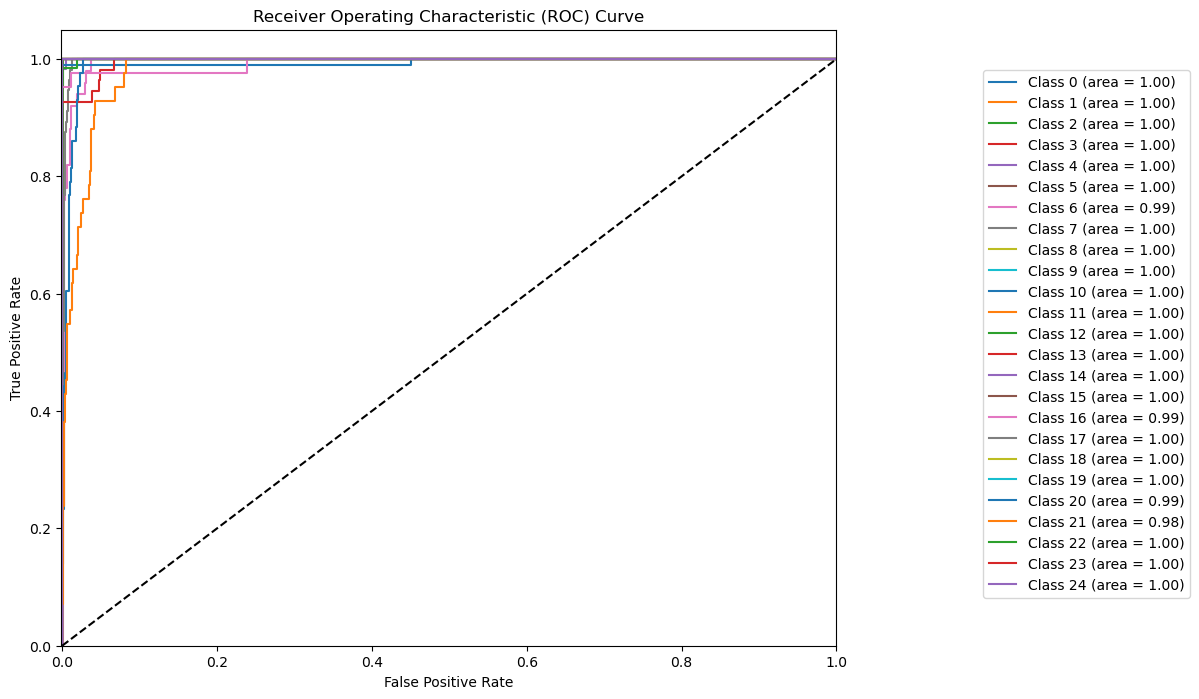
\includegraphics[width=0.8\linewidth]{images/final/roc.png}
  \caption{AUC-ROC Curve of Final Model\\AVG ROC AUC: 0.99814}
  \label{aff}
\end{figure}

The above three images show the AUC-ROC curves for each model, with a true positive rate (TPR) vs false positive rate (FPR) graph. The most optimal shape presented would be a straight corner shape, which would signify that there were no false positives at all, and every prediction was correct, with a 100\% true positive rate. As usual, parallel with previous results, the starter model had the worst run, with the curve being all over the place. Many of the runs had a high false positive rate, with one nearing 60\%. This shows us that this specific model, in some cases, can have up to 60\% false positives, becoming very unreliable. On the other hand, the revised and final models have very similar charts, indicating that both performances were on par, with lines being near the optimal shape. However, the average ROC AUC scores are very similar, only varying in the thousandths place. This is due to how many other lines are perfectly optimal, with the corner curve, which can inflate the scores.
%---------------------------------------------------------------------------------------------------------------------------------

\section{Conclusion}
\subsection{Results}

Our testing with these models have created a standard for how the convolutional neural network performs for the purpose of classifying malware. What we found was that was having more layers generally increases performance, however, not to an excess. Models such as the starter model, which only have a minimal number of layers can be seen doing significantly worse in F1-Score, Recall, Precision, AUC ROC Score + Curve. However, this model has higher consistency with the accuracy graph, which can propose that an increase of layers may allow for better quality predictions, but can also lead to inconsistency in results, or overfitting.

Our best results came from the final model, as it was the most optimized and fine tuned. It boasted high scores across all performance metrics, showing that it was able to predict malware images with high accuracy. Each incremental model, (starter, revised, and final) showed improvement, in which we were able to use their reported metrics as feedback to adjust for optimization. One thing that we could of done better would be to better evaluate our models on various datasets, instead of just one. This could give us a wide variety of results, and allow us to see how each model interacts with different malware images.

Our plan going forward will now be to expand the models we will use. In this case, we use a convolutional neural network, but we are planning to use models such as ResNet, EfficientNet, VGG-16, and Inception. Furthermore, with the addition of these newer models, we will also be adding other datasets, to be able to test on a wide variety of criteria and types of malware. By being able to use specially trained AI models to classify malware, it will allow many of the modern day issues with malware classification be solved.

\bibliographystyle{IEEEtran}
\bibliography{ref}

\end{document}
 